\documentclass[]{article}
\usepackage{lmodern}
\usepackage{amssymb,amsmath}
\usepackage{ifxetex,ifluatex}
\usepackage{fixltx2e} % provides \textsubscript
\ifnum 0\ifxetex 1\fi\ifluatex 1\fi=0 % if pdftex
  \usepackage[T1]{fontenc}
  \usepackage[utf8]{inputenc}
\else % if luatex or xelatex
  \ifxetex
    \usepackage{mathspec}
  \else
    \usepackage{fontspec}
  \fi
  \defaultfontfeatures{Ligatures=TeX,Scale=MatchLowercase}
\fi
% use upquote if available, for straight quotes in verbatim environments
\IfFileExists{upquote.sty}{\usepackage{upquote}}{}
% use microtype if available
\IfFileExists{microtype.sty}{%
\usepackage{microtype}
\UseMicrotypeSet[protrusion]{basicmath} % disable protrusion for tt fonts
}{}
\usepackage[margin=1in]{geometry}
\usepackage{hyperref}
\hypersetup{unicode=true,
            pdfborder={0 0 0},
            breaklinks=true}
\urlstyle{same}  % don't use monospace font for urls
\usepackage{graphicx,grffile}
\makeatletter
\def\maxwidth{\ifdim\Gin@nat@width>\linewidth\linewidth\else\Gin@nat@width\fi}
\def\maxheight{\ifdim\Gin@nat@height>\textheight\textheight\else\Gin@nat@height\fi}
\makeatother
% Scale images if necessary, so that they will not overflow the page
% margins by default, and it is still possible to overwrite the defaults
% using explicit options in \includegraphics[width, height, ...]{}
\setkeys{Gin}{width=\maxwidth,height=\maxheight,keepaspectratio}
\IfFileExists{parskip.sty}{%
\usepackage{parskip}
}{% else
\setlength{\parindent}{0pt}
\setlength{\parskip}{6pt plus 2pt minus 1pt}
}
\setlength{\emergencystretch}{3em}  % prevent overfull lines
\providecommand{\tightlist}{%
  \setlength{\itemsep}{0pt}\setlength{\parskip}{0pt}}
\setcounter{secnumdepth}{0}
% Redefines (sub)paragraphs to behave more like sections
\ifx\paragraph\undefined\else
\let\oldparagraph\paragraph
\renewcommand{\paragraph}[1]{\oldparagraph{#1}\mbox{}}
\fi
\ifx\subparagraph\undefined\else
\let\oldsubparagraph\subparagraph
\renewcommand{\subparagraph}[1]{\oldsubparagraph{#1}\mbox{}}
\fi

%%% Use protect on footnotes to avoid problems with footnotes in titles
\let\rmarkdownfootnote\footnote%
\def\footnote{\protect\rmarkdownfootnote}

%%% Change title format to be more compact
\usepackage{titling}

% Create subtitle command for use in maketitle
\providecommand{\subtitle}[1]{
  \posttitle{
    \begin{center}\large#1\end{center}
    }
}

\setlength{\droptitle}{-2em}

  \title{}
    \pretitle{\vspace{\droptitle}}
  \posttitle{}
    \author{}
    \preauthor{}\postauthor{}
    \date{}
    \predate{}\postdate{}
  
\pagenumbering{gobble}
\usepackage{placeins}
\usepackage{float}
\usepackage{caption}
\captionsetup[figure]{labelformat = empty}
\usepackage{xcolor}
\definecolor{link}{rgb}{0, 0, 238}
\usepackage{booktabs}

\begin{document}

{
\setcounter{tocdepth}{5}
\tableofcontents
}
\hypertarget{critical-element-2---assessment-system-operations}{%
\subsection{Critical Element 2 - Assessment System
Operations}\label{critical-element-2---assessment-system-operations}}

\hypertarget{test-design-and-development}{%
\subsubsection{2.1 Test Design and
Development}\label{test-design-and-development}}

The test specifications document that describes our approach to
assessment and test design for the ORExt is published in \emph{Appendix}
2.1. The document includes our approach to reducing the depth, breadth,
and complexity (RDBC) of grade level content standards, an overview of
the essentialization process and EAF documents, the planned test design
for the ORExt, test development considerations, sample test items, item
specifications, and universal tools/designated supports/accommodations.
Only Grade 7 Math field test items were developed in 2017-18 which were
in accordance with the 2014-15 test specifications, and are the most
current available.

\hypertarget{a-orext-purpose}{%
\paragraph{2.1A ORExt Purpose}\label{a-orext-purpose}}

The stated purpose of the ORExt is to provide the state technically
adequate student performance data to ascertain proficiency on grade
level state content standards for students with significant cognitive
disabilities. A long-term goal of the program is to also provide
information regarding annual student growth related to these content
standards over Grades 3-8, as measured by vertically scaled assessments
in ELA and Mathematics. The results of the assessment are currently
reported in comparison to four performance levels: Level 1, Level 2,
Level 3, and Level 4. Levels 3 and 4 denote a proficient level of
performance, while Levels 1 and 2 denote performance that is not
proficient. BRT and ODE developed a scaled score interpretation guide to
assist stakeholders in interpreting the meaning of the scaled scores
generated by the ORExt, supported by the state's achievement level
descriptors. This guidance is published in \emph{Appendix} 2.1A.

\hypertarget{b-orext-test-blueprint}{%
\paragraph{2.1B ORExt Test Blueprint}\label{b-orext-test-blueprint}}

\emph{Appendix} 2.1B includes the entire test blueprint for the ORExt,
as conveyed by the balance of representation across content areas and
domains. Field-testing is conducted each year in order to support the
continuous improvement of test functioning. However, items are selected
to maintain this balance of representation. Oregon teachers validated
the content of the assessment, agreeing with the standards that were and
were not selected to develop the Essentialized Standards to which the
ORExt test items are aligned.

\hypertarget{c-test-development-processes}{%
\paragraph{2.1C Test Development
Processes}\label{c-test-development-processes}}

The test development process implemented for the ORExt is conveyed in
\emph{Appendix} 2.1C, including standard selection and validation, item
development, item review, review of all Oregon teacher feedback and
updating of items, and scaling and item selection. The \emph{Appendix}
articulates the process used to generate the materials with comma
separated value files used to create item templates that fed into Adobe
InDesign© through a data merge. Final test packages are reviewed for
accuracy and content and then disseminated via secure file transfer to
Oregon Qualified Assessors.

\hypertarget{d-computer-adaptive-considerations}{%
\paragraph{2.1D Computer-Adaptive
Considerations}\label{d-computer-adaptive-considerations}}

The ORExt is not a computer-adaptive instrument, so these concerns do
not apply.

\hypertarget{item-development}{%
\subsubsection{2.2 Item Development}\label{item-development}}

Item writers were recruited by ODE staff using an existing Qualified
Assessor/Qualified Trainer listserv. \FloatBarrier
\includegraphics{Figures/ItemDev/ItemDev.png}

\hypertarget{project-description}{%
\paragraph{Project Description:}\label{project-description}}

Behavioral Research and Teaching at the University of Oregon recruited
Oregon teachers to participate in item development for a new alternate
assessment. Selected teachers were asked to develop 360 items in English
Language Arts, Mathematics, or Science over the course of the summer,
from mid-June through end of August. The Project Director worked with
lead item developers to provide training, ongoing review and feedback,
and quality assurance. All participants were expected to provide
documentation of their qualifications and sign test security agreements.
In addition, all item developers were expected to participate in a
half-day item development training based upon the following schedule:
ELA - Tuesday, from 8 AM to 12 PM; Math - Wednesday, from 8 AM to 12 PM;
Science - Thursday, from 8 AM to 12 PM.

\hypertarget{minimum-qualifications}{%
\paragraph{Minimum Qualifications:}\label{minimum-qualifications}}

All licensed Oregon public school teachers with at least three years of
teaching in a life skills/severe needs program (SPED) or a general
education classroom (GEN-ED), respectively, were encouraged to apply.
Preference was given for item writing experience, additional years of
teaching experience, and higher education degree status.

\hypertarget{compensation}{%
\paragraph{Compensation:}\label{compensation}}

Teachers who participated in this process were compensated at a rate of
\$20/hr via professional service contracts. It was anticipated that
teachers would produce 4 ELA items/hr, 6 Science items/hr, and 8 Math
items/hr. As such, the maximum contract amount for ELA was \$1,800, for
Science \$1,440, and for Math \$900. Item development focused primarily
on writing the stem and 3 options, with no need to produce graphics
(rather use labels for a BRT graphic designer to produce).

\hypertarget{contact}{%
\paragraph{Contact:}\label{contact}}

Because the timeline required work over the summer, Oregon teacher
recruitment was challenging. BRT researchers thus performed an
additional on-campus recruitment within the College of Education using
the same information. The final pool of item writers included 18 item
writers: seven Oregon teachers (all with MA degrees), five PhD
candidates within the COE, and six BRT researchers (four PhD candidates,
one PhD, and one with an MA). Item writers averaged 11.5 years of
teaching experience. The teachers recruited all had prior experience
developing items for the ORExt, as did all of the BRT researchers. The
five PhD candidates within the COE had no prior item development
experience. All item development was reviewed by BRT researchers and the
Project Manager.

The item development process followed is elaborated in \emph{Appendix}
2.2.1, which is the PowerPoint used in training all Oregon item writers.
The item development process was structured with the following steps.
Item writers were first oriented to the student population, as the pool
of item writers included both content and special education experts. The
Essentialization Process used to RDBC grade level standards was then
modeled so writers would understand how the item alignment targets, the
Essentialized Standards, were generated. Lecture, guided practice, and
independent practice activities and follow-up discussion ensured
comprehension of the process. BRT staff developed exemplar items for
every Essentialized Standard, varying the complexity from Low (L) to
Medium (M) to High (H) levels of complexity to convey the different
performance expectations at each level. The balanced vertical scaling
design provided an overall form-to-form and grade-to-grade level
framework for the test formation process once items were developed (see
\emph{Appendix} 2.2.2). Sample items are provided in \emph{Appendix}
2.2.3 for stakeholder reference, demonstrating the format and style of
typical items on the ORExt.

\hypertarget{test-administration}{%
\subsubsection{2.3 Test Administration}\label{test-administration}}

The ORExt assessments are administered according to the administration,
scoring, analysis, and reporting criteria established in the ORExt
General Administration Manual (see \emph{Appendix} 2.3). Important
updates to the testing process are distributed via the
\color{link}\href{http://www.oregon.gov/ode/educator-resources/assessment/Pages/Assessment-and-Accountability-Update.aspx}{Assessment
and Accountability Updates} \color{black} listserve, as well. ODE uses
this system to communicate information that is relevant for the
statewide assessment system, including the ORExt. Announcements are sent
to the listserv by email and are also posted to the ODE website. The
standardization of test administration is supported by a comprehensive
training process described below in Section 2.3B.

\hypertarget{a-administration-and-accommodations}{%
\paragraph{2.3A Administration and
Accommodations}\label{a-administration-and-accommodations}}

The state has ensured that appropriate universal tools, designated
supports, and accommodations are available to students with disabilities
and students covered by Section 504 by providing guidance and technical
support on accommodations (see \emph{Appendices} 2.3A.1 and 2.3A.2).
Guidelines regarding use of the accommodations for instructional
purposes are included in the document, as all students are expected to
receive test accommodations that are consistent with instructional
accommodations.

Accommodations are built into the flexibility provided by the ORExt test
though they have not yet been researched for the ORExt. However, annual
training and proficiency testing efforts related to becoming a qualified
assessor and/or qualified trainer for the ORExt support standardized use
of available accommodations that are not already part of the test
design. Based on annual analyses, results demonstrate that student
performance varies according to their abilities and not
construct-irrelevant factors, such as sex, race, or ethnicity (See
Section 4.2).

The state has ensured that appropriate accommodations are available to
students with limited English proficiency by providing guidance and
technical support on accommodations (see \emph{Appendix} 2.3A.1).
Communication systems for this student population are limited; exposure
to multiple languages can make a student's communication system more
complex. The ORExt uses universal design principles and simplified
language approaches in order to increase language access to test content
for all students. In addition, directions and prompts may be
translated/interpreted for students in their native language.

An analysis of accommodated versus non-accommodated administrations is
needed in order to demonstrate that the provision of language
accommodations is not providing any advantage to students with limited
English proficiency, nor any disadvantage to other participants.
Accommodations information was collected this year as an option for data
entry. Entering accommodations information will be required next year.
Analyses of the impact of accommodation provision on the ORExt should
thus be feasible after the spring 2019 administration.

The Oregon Extended assessments can be administered using both Large
Print and Braille (contracted and non-contracted) versions, as well.
Oregon has ensured that the Oregon Extended assessments provide an
appropriate variety of accommodations for students with disabilities.
The state has provided guidance on accommodations in presentation,
response, setting, and timing in the Accommodations Manual 2013-14: How
to Select, Administer, and Evaluate Accommodations for Oregon's
Statewide Assessments (see \emph{Appendix} 2.3A.2). The Oregon Extended
assessments are also designed according to universal design principles
and utilize a simplified language approach (see \emph{Appendix} 2.3A.3).

In the 2013-2014 school year, the state developed a training and
proficiency program for sign language interpretation of its assessments
and has updated the site annually since that time. The
\color{link}\href{http://lms.brtprojects.org}{sign language training}
\color{black} process included videos of interpreters administering
items to students, materials that support appropriate administration
(i.e., transcripts and PowerPoint slides that supplement the video
administrations and the current ODE accommodations manual), and
proficiency testing to support standardized interpretation for Oregon's
assessments, including the ORExt. A 10-item proficiency test was
administered, with an 80\% required for passing (8/10 items correct). In
2017-18, the site was used to train 61 participants. All participants
passed the assessment on the first attempt. The overall average score on
the proficiency test was 95.9\%.

The ORExt assessments provide an appropriate variety of linguistic
accommodations for students with limited English proficiency. They also
use a simplified language approach in test development in order to
reduce language load of all items systematically (see \emph{Appendix}
2.3A3). Any given student's communication system may include home signs,
school signs, English words, and Spanish words, for example. With the
exception of items that require independent reading, the ORExt
assessment can be translated or interpreted by a Qualified Assessor (QA)
working with an interpreter in the student's native language, including
American Sign Language. QAs are allowed to translate/interpret the test
directions. QAs can adapt the assessment to meet the needs of the
student, while still maintaining standardization due to systematic
prompts and well-defined answers.

\hypertarget{b-comprehensive-training-system}{%
\paragraph{2.3B Comprehensive Training
System}\label{b-comprehensive-training-system}}

Comprehensive information for ongoing training for all qualified
assessors (QAs) and Qualified Trainers (QTs) is provided in
\emph{Appendices} 2.3B.1-2.3B.8. Through an online distribution and
assessment system, \color{link}\href{https://or.k12test.com/}{QA/QT
Training and Proficiency} \color{black} is determined anually. This
website hosts all resources and information needed to administer, score,
report, and interpret the results from the ORExt. The website also
includes proficiency assessments that are required for all QAs and QTs
who may administer the ORExt. QTs are directly trained by ODE and BRT
staff as part of a train the trainers model. QTs then provide direct
trainings for new QAs in their respective regions.

The Oregon Department of Education (ODE) provided four direct statewide
trainings for new Qualified Trainers (QTs) and Qualified Assessors (QAs)
in face-to-face regional trainings. The schedule for the regional
trainings, as well as relevant training information, is provided below:
\FloatBarrier
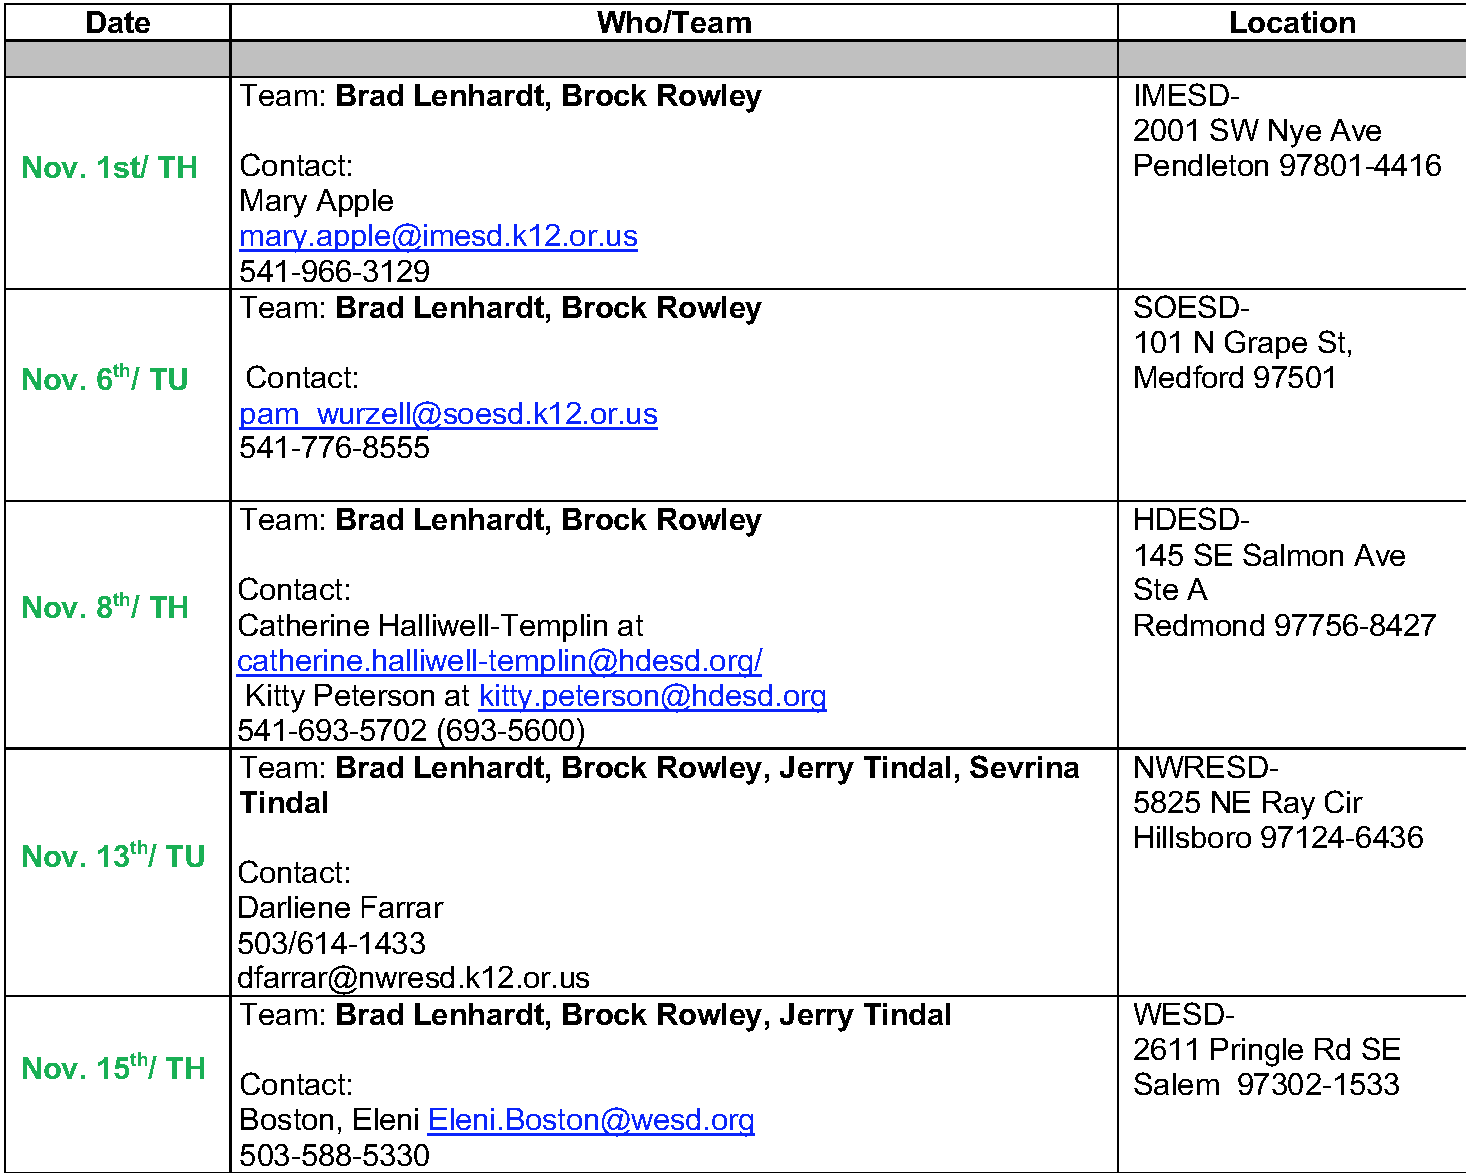
\includegraphics{Figures/TrainingSched/2018_19_TrainingSchedule.png}

Only trained Qualified Assessors (QAs) can administer the Oregon
Extended assessment. Qualified Assessors who also receive direct
instruction from ODE and BRT may become Qualified Trainers (QTs) who are
certified to train local staff using the train-the-trainers model.
Training for new assessors must be completed on an annual basis.
Assessors who do not maintain their respective certifications for any
given year must re-train if they choose to enter the system again.

The tables below contain data from the
\color{link}\href{http://or.k12test.com/}{Oregon Extended Assessment
Training and Proficiency Website}\color{black}. All assessors need to
complete some form of training each year to retain their status for
administering the Extended Assessments.

New assessors and returning assessors who needed further training in
2017-18 were required to pass four proficiencies with a score of 80\% or
higher. These four proficiencies were in Administration, English
Language Arts (ELA), Mathematics, and Science. Returning QAs or QTs for
the 2017-18 school year only needed to pass a Refresher Proficiency,
again with a score of 80\% or higher. The tables below contain data on
the number of assessors (participants) in each of the four
proficiencies, as well as the Refresher Proficiency. Included in the
data is the number of attempts needed to attain a passing score as well
as the average passing score of the participants.

An analysis of the Oregon Extended Assessment Training and Proficiency
Website showed 377 Assessors in-Training, 928 Qualified Assessors, and
137 Qualified Trainers registered with the system. \FloatBarrier
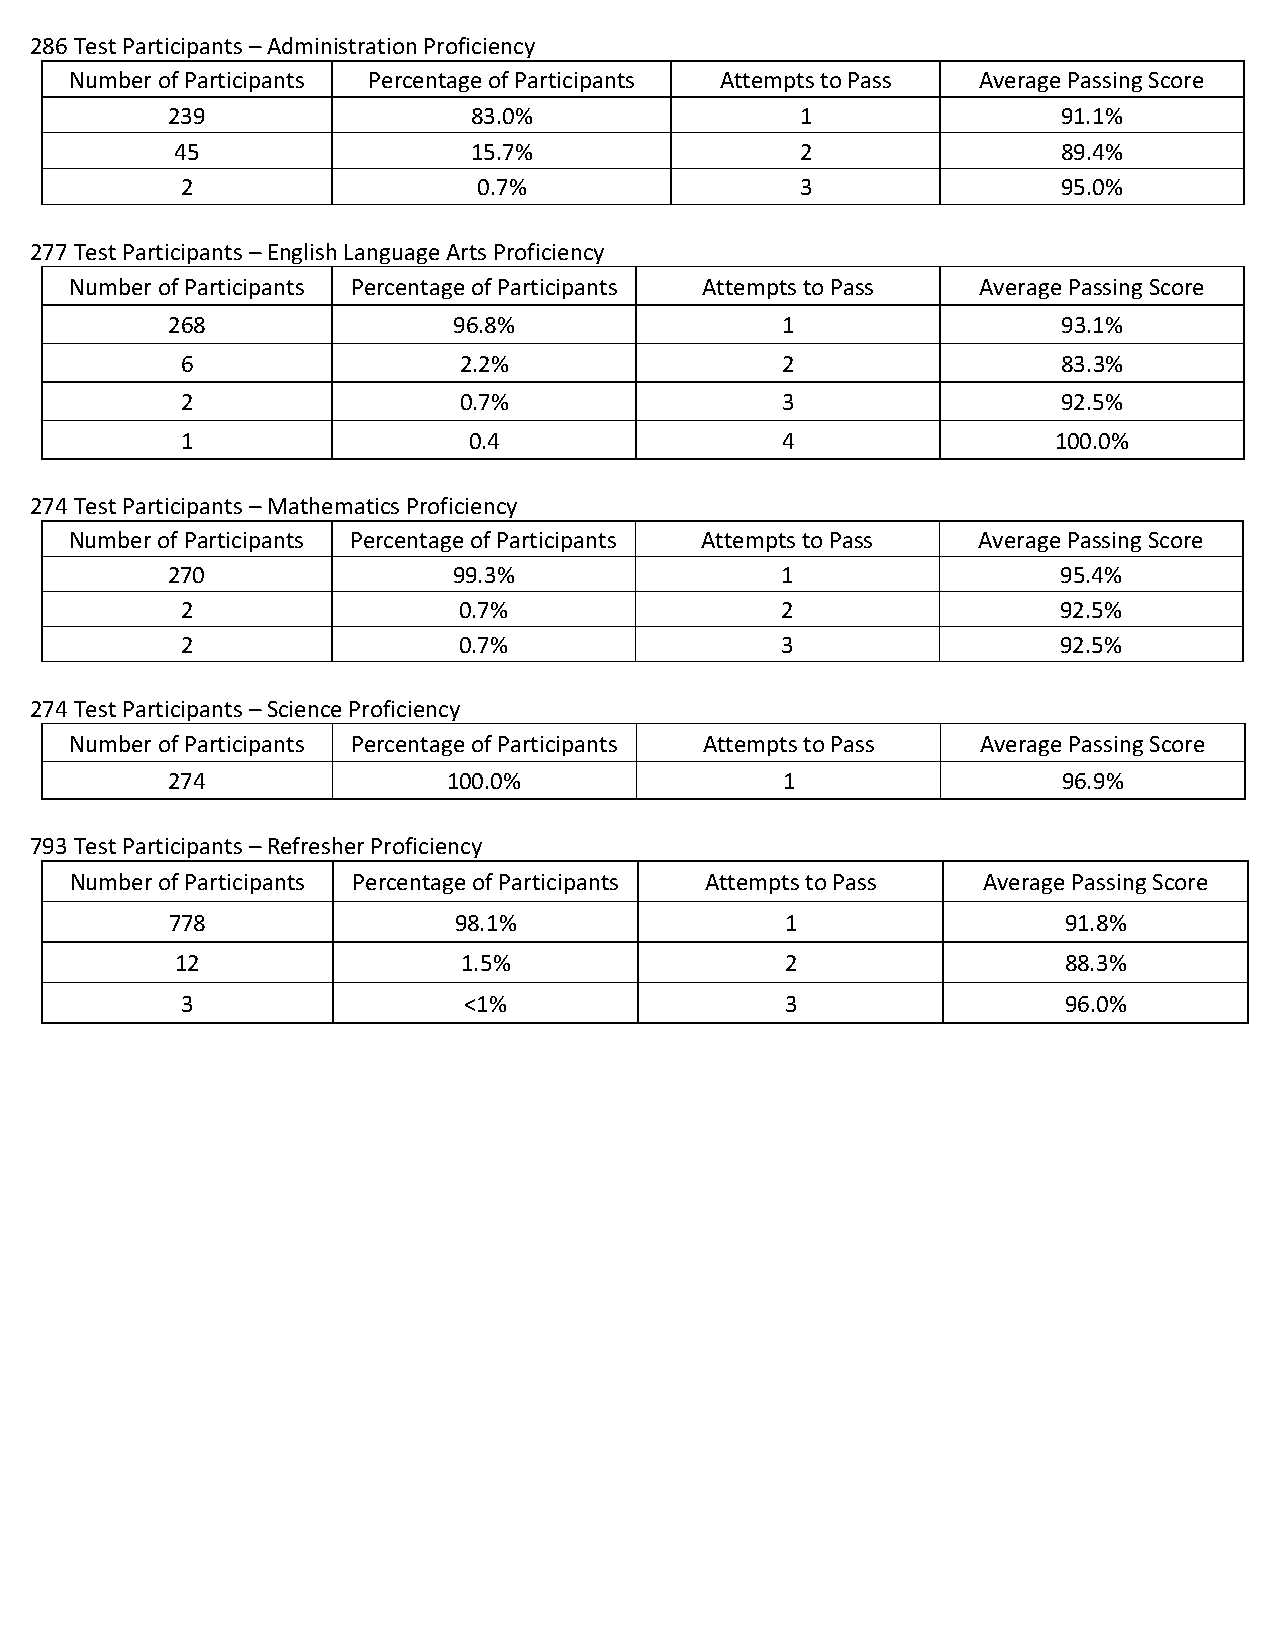
\includegraphics{Figures/TestPartic/QA_QT_TestPartic_1819}

A higher number of assessors completed the Refresher Proficiency test
than the subject area proficiency tests reflecting a greater number of
return assessors compared to new assessors. Data showed ELA Proficiency
to be the most challenging to new assessors, but most were able to pass
on the first or second attempt with about 1\% or less of assessors
requiring more than two attempts and science to be the least challenging
with 100\% of assessors passing on the first attempt. The majority of
assessors passed the Administration and Math proficiency tests on the
first and second attempts with less than 1\% requiring a third attempt.
The majority of returning assessors passed the refresher on the first
attempt with less than 2\% requiring a seond and third attempt. There
were 12 fewer Qualified Assessors and 2 more Qualified Trainers compared
to last year.

Evaluations are collected at each QT training in November. The results
reflect general approval, but also suggest areas of improvement that ODE
and BRT work on for subsequent trainings/subsequent years, as
appropriate. QT evaluations this year included positively worded
statements regarding the quality of training rated on a scale where 1 =
Strongly Disagree, 2 = Disagree, 3 = Agree, and 4 = Strongly Agree.

The first section evaluated the state-level information and the
knowledge of the ODE presenters, the participants' level of comfort with
the training provided, the participants' ability to carry this training
and materials back to train district staff, and the overall utility of
the training. Eighty four percent of participants strongly agreed with
these statements, fourteen percent agreed, and less than one percent
disagreed and strongly disagreed, collectively. In the second section,
participants were asked to evaluate the BRT trainers and their
guidelines regarding how to use the training and proficiency website and
related resources. Eight three percent of participants strongly agreed
with these statements, sixteen percent agreed, and less than one percent
disagreed and strongly disagreed, collectively. Overall, these results
demonstrate that participants felt that the training was high quality
and they felt confident that they could train their staff upon return to
their respective districts with the knowledge and resources gained. This
year's QT training cycle included an optional afternoon session for any
interested educators on how to essentialize grade level content
standards and how to develop curriculum and provide instruction that is
aligned to those standards for students who are functioning off grade
level, with a focus on students with significant cognitive disabilities
(SWSCD).

In addition, all technical assistance questions that we receive from the
field as part of our HelpDesk are documented. The most common inquiries
for the 2018-19 test administration window involved credential
verification to add schools/students to rosters, selecting appropriate
IDEA disability codes for rosters, and manual grading for the electronic
ELA writing items. Some other common inquiries included exit PIN, access
to monitoring for DTC's, and technical issues with individual tablet.
All helpdesk inquiries will be taken into consideration as the training
site is updated for the 2019-2020 testing year.

Oregon monitors the quality of its system in several ways in order to
support continuous improvement. In terms of the assessment quality, item
statistics are reviewed each year and items that are not functioning as
intended are removed and replaced by better functioning field-test
items.

In 2014-15, items were reviewed in two phases, first using classical
test theory (CTT) and second using Rasch analyses. All items flagged as
a result of the statistical reviews were analyzed, item-by-item, by a
team of measurement and content experts at BRT. Not all flagged items
were removed, as several did not have apparent design flaws.
Considerations regarding domain representation as well as item
difficulty range also were considered during the review process. We also
employed different decision rules for unique items versus horizontally-
or vertically-scaled anchor items. It was important in many cases to
maintain anchor items. Items with clear design flaws were removed from
subsequent analyses and reporting. The following flagging criteria were
employed:

\begin{itemize}
\tightlist
\item
  \textbf{CTT}: A unique item was flagged if it had a p-value of .10 or
  lower, .90 or higher, or a point biserial \textless{} .15. Anchor
  items were flagged if they had a p-value of .10 or lower or .95 and
  higher on all forms or a point biserial \textless{} .45 on any form.
\item
  \textbf{Rasch}: Unique items were flagged if their outfit mean square
  values were between 0 and .25 or \textgreater{} 1.5. Anchor items were
  flagged if their outfit mean square values were \textless{} .5,
  \textgreater{} 1.8 for horizontal items, or \textgreater{} 2.0 for
  vertical anchor items.
\end{itemize}

Out of a total of 5,929 items developed in 2014-15, 166 were removed
(2.8\%).

We also implement a consequential validity study each year that surveys
QAs and QTs regarding the academic and social consequences of the ORExt,
both intended and unintended. The Consequential Validity report is
published in \emph{Appendix} 2.3B.10. ODE and BRT staff review the
results of the survey annually to determine what program improvements
are needed. A summary of the results is provided below.

ODE implemented a research survey program to address the need to
document the consequences, both intended and unintended, of the ORExt
Assessments. The research questions have been framed based upon current
consequential validity approaches for alternate assessments in the
literature, as well as issues that are of specific value in Oregon. The
survey included 121 respondents. This was 11\% of the solicited
respondents, who were all Qualified Assessors (QAs) and Qualified
Trainers (QTs) in the or.k12test.com database. The sample was 83\%
female and represented all regions of the state, as well as age ranges.
The survey included a range of quantitative and qualitative components.
The quantitative results demonstrate that QAs and QTs continue to feel
that the ORExt test items were easy to administer and score (64.2\%
Strongly Agree) and felt confident in their ability to interpret scaled
scores and Achievement Level Descriptors for the ORExt (69.8\% Strongly
Agree and Agree). They also felt that the items were accessible for
students who participated (78\% Strongly Agree and Agree) and that the
ORExt reflected the academic content that SWSCD should be learning
(68.4\% Strongly Agree and Agree). QAs and QTs felt marginally positive
about the educational impacts of the ORExt and marginally negative about
its social impacts. The results again demonstrate that the ORExt content
area assessments generally require up to one hour to administer.

The qualitative results revealed two areas in which educators
appreciated the ORExt and four areas of needed improvement. QAs and QTs
said that they appreciated: 1) the assessment's efficiency (i.e., more
streamlined administration, ease of administration, easier to give and
score online, online materials distribution); and, 2) overall item and
test design (i.e., one item per page, visual supports, scoring protocol
and student materials design, accessibility of test questions). Teachers
recommended the following areas of improvement, not all of which are
actionable: 1) Option to administer the assessment electronically, 2) A
functional skills assessment, 3) New items for very low functioning
students should be developed, and 4) A math assessment composed of more
practical/life skills problems involving time and money. Complete
results, including anticipated responses, from the survey can be found
in \emph{Appendix} 2.3B.10.

\hypertarget{c-technology-based-assessments}{%
\paragraph{2.3C Technology-based
Assessments}\label{c-technology-based-assessments}}

The ORExt was implemented using a technology-based platform as Phase 3
of the ORExt Tablet Administration. The 2017-18 testing window was the
first year all grade level and subject area assessments were available
on the electronic application/web-based platform. Administration of the
electronic application mirrors paper/pencil administration with each
item read aloud to the student, and the student asked to select one of
three answer choices. Electronic based functionality includes optional
discontinuation if the student misses 10 out of the first 15 items,
directing the assessor to administer the ORora. To support understanding
of the system by both teachers and students, a separate practice test
application is available. Helpdesk inquiries and feedback from the field
indicated much preference of the electronic administration versus
paper/pencil. Qualified Trainers and Qualified Assessors reported their
students' were more focused during electronic administration, and
because the application scores automatically it was much more efficient
for assessors. Improvements will be made to the electronic test based on
technology improvements and feedback from the field. Data entry for all
platforms is now maintained and monitored by secure BRT servers.

\hypertarget{monitoring-test-administration}{%
\subsubsection{2.4 Monitoring Test
Administration}\label{monitoring-test-administration}}

The ODE maintains a rigorous training system to support standardized
test administration for the \color{link}
\href{https://or.k12test.com}{Oregon K12 website}\color{black}, (secure
website, but see screenshot below for an example of training content).
\FloatBarrier
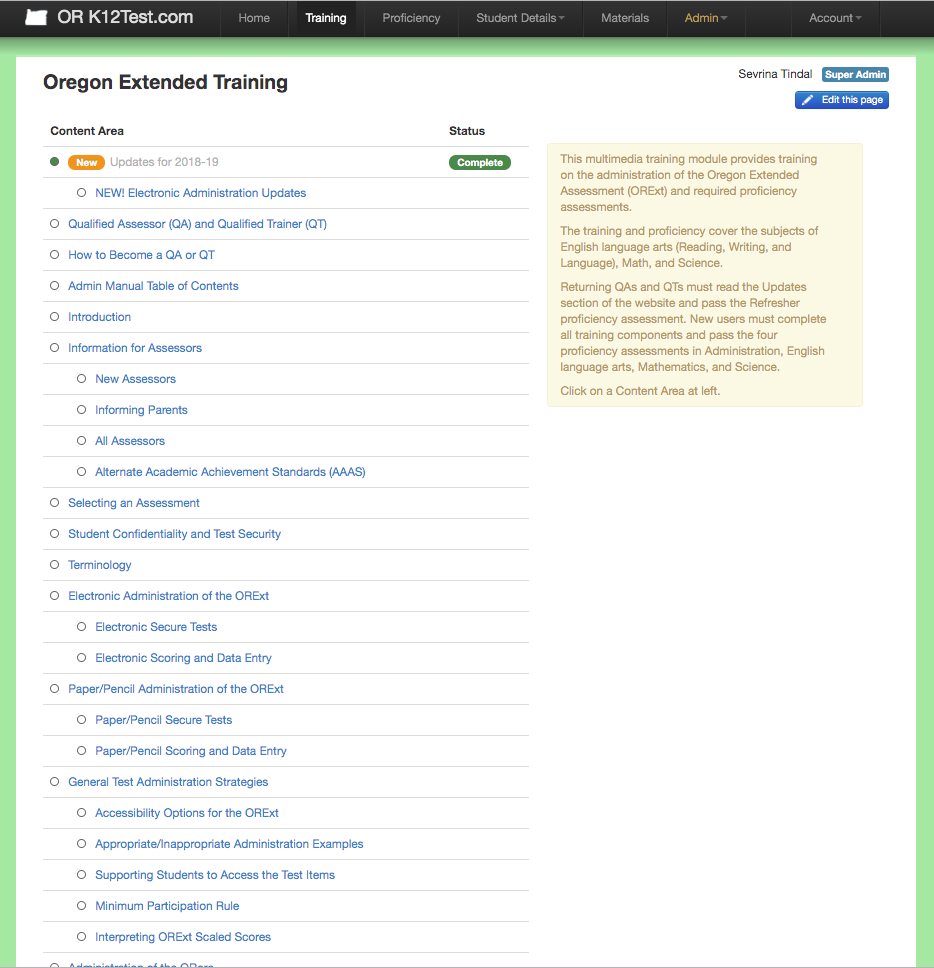
\includegraphics{Figures/TrainingSite/TrainingSiteContentExample.png}

The or.k12test.com website includes a training section that addresses
any systems updates, the process for becoming a Qualified Assessor or
Qualified Trainer, student eligibility expectations, student
confidentiality and test security, test administration and scoring
expectations, examples of appropriate and inappropriate administration
(video), supporting student access to items without violating the test
construct, content area trainings that demonstrate how to administer
items in ELA, Math, and Science (video, with supporting test materials),
and how to access secure tests and complete data entry. Information for
QAs, QTs, and parents regarding the ORExt is also provided, as are all
necessary support materials. For QAs, these materials include practice
tests to prepare both themselves and students for the annual assessment
and all of the training materials used on the website. In addition to
these materials, QTs have access to all training materials necessary to
provide annual training to QAs in their purview (see screenshot below):
\FloatBarrier 
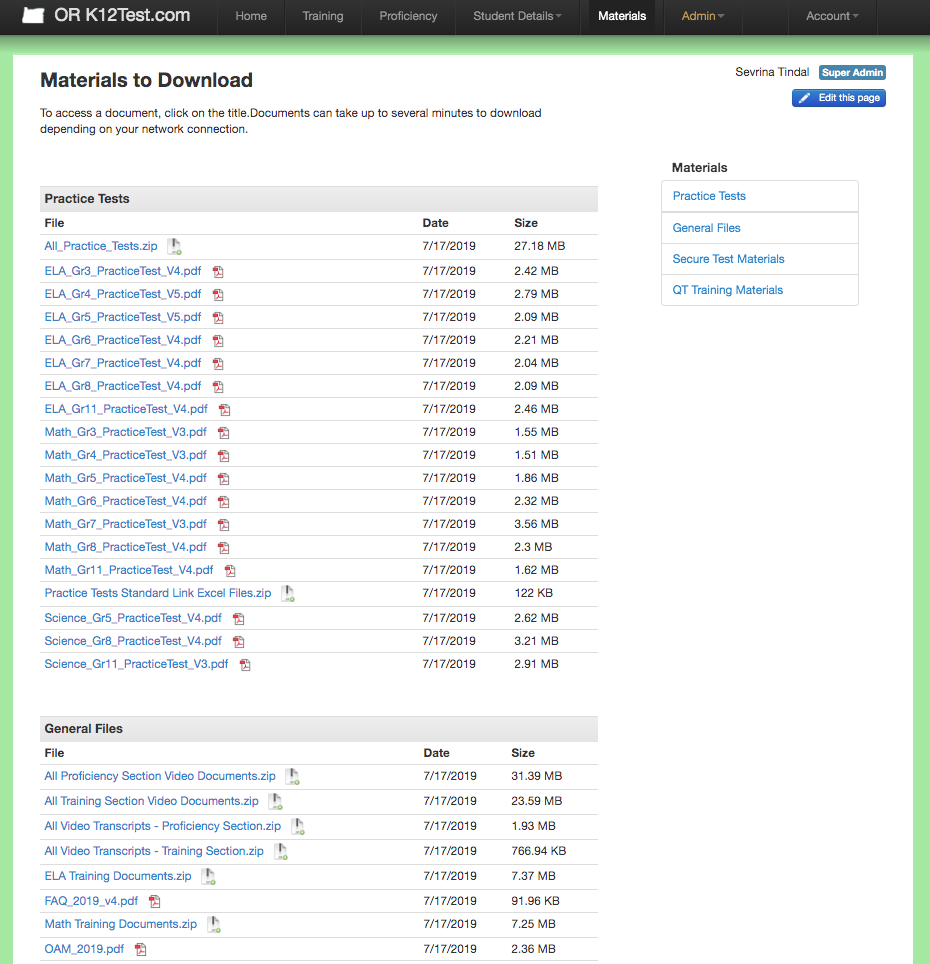
\includegraphics{Figures/TrainingSite/MaterialsToDownload.png}

In addition, monitoring and reporting related to test administration
issues for the ORExt is addressed via general ODE reporting systems.
Information regarding this process can be located in the general
assessment system Peer Review evidence submission.

\hypertarget{test-security}{%
\subsubsection{2.5 Test Security}\label{test-security}}

\hypertarget{a-prevention-of-assessment-irregularities}{%
\paragraph{2.5A Prevention of Assessment
Irregularities}\label{a-prevention-of-assessment-irregularities}}

Test security policies and consequences for violation are addressed in
the Test Administration Manual on an annual basis (see \emph{Appendix}
1.4.2, p.~29-33). These policies include test material security, proper
test preparation guidelines and administration procedures, consequences
for confirmed violations of test security, and annual training
requirements at the district and school levels for all individuals
involved in test administration. Consequences for adult-initiated test
irregularities may be severe, including placing teaching licenses in
jeopardy (see \emph{Appendix} 1.4.2, p.~31-33).

\hypertarget{b-detection-of-test-irregularities}{%
\paragraph{2.5B Detection of Test
Irregularities}\label{b-detection-of-test-irregularities}}

The ODE utilizes a localized monitoring system where school test
coordinators oversee building-level administration by trained, Qualified
Assessors, and report to centralized district test coordinators, who are
then responsible for reporting any confirmed violations to ODE.
Improprieties are defined as adult-initiated or student-initiated and
investigated accordingly (see \emph{Appendix} 1.4.2, p.~29-31).

\hypertarget{c-remediation-following-test-security-incidents}{%
\paragraph{2.5C Remediation Following Test Security
Incidents}\label{c-remediation-following-test-security-incidents}}

ODE's alternate assessment program manager investigates and remediates
substantiated test security incidents for the ORExt by working with
district test coordinators. Additional information regarding this
process can be located in the general assessment system Peer Review
evidence submission.

\hypertarget{d-investigation-of-test-irregularities}{%
\paragraph{2.5D Investigation of Test
Irregularities}\label{d-investigation-of-test-irregularities}}

School and district test coordinators conduct initial investigations
into all alleged test irregularities. Once reported to ODE, all alleged
test irregularities are investigated in consultation with district test
coordinators and the test vendor, as appropriate (see \emph{Appendix}
1.4.2, p.~31-33). In the event that a test irregularity is determined to
be factual, consequences are determined based upon contextual issues
that are brought to light during the investigation. Additional
information regarding this process can be located in the general
assessment system Peer Review evidence submission.

\hypertarget{systems-for-protecting-data-integrity-and-privacy}{%
\subsubsection{2.6 Systems for Protecting Data Integrity and
Privacy}\label{systems-for-protecting-data-integrity-and-privacy}}

\hypertarget{a-integrity-of-test-materials}{%
\paragraph{2.6A Integrity of Test
Materials}\label{a-integrity-of-test-materials}}

Test materials for the ORExt are maintained throughout development,
dissemination, and administration via multiple mechanisms. All items
under development are stored in secure file servers managed by
Behavioral Research \& Teaching at the University of Oregon, the test
vendor for the ORExt. Item reviews necessary to provide alignment, bias,
and sensitivity information are conducted online using the secure
\color{link}\href{http://brtitemreview.com}{Distributed Item Review
(DIR)}\color{black} platform (secure website, but see \emph{Appendix}
3.1B for a system overview).

For the 2018-2019 school year, all paper/pencil secure test distribution
and data entry was hosted by BRT through the secure training site.

The secure tablet application and web-based platform distribution and
data entry were hosted by BRT servers. All technology based secure
administration and data entry was password-protected. Download of the
tablet app was dependent on the type of device, all instructions and
download links were available in the Test App User Guide (see
\emph{Appendix} 2.6A) Additional information regarding test security can
be located in the general assessment system Peer Review evidence
submission. \FloatBarrier
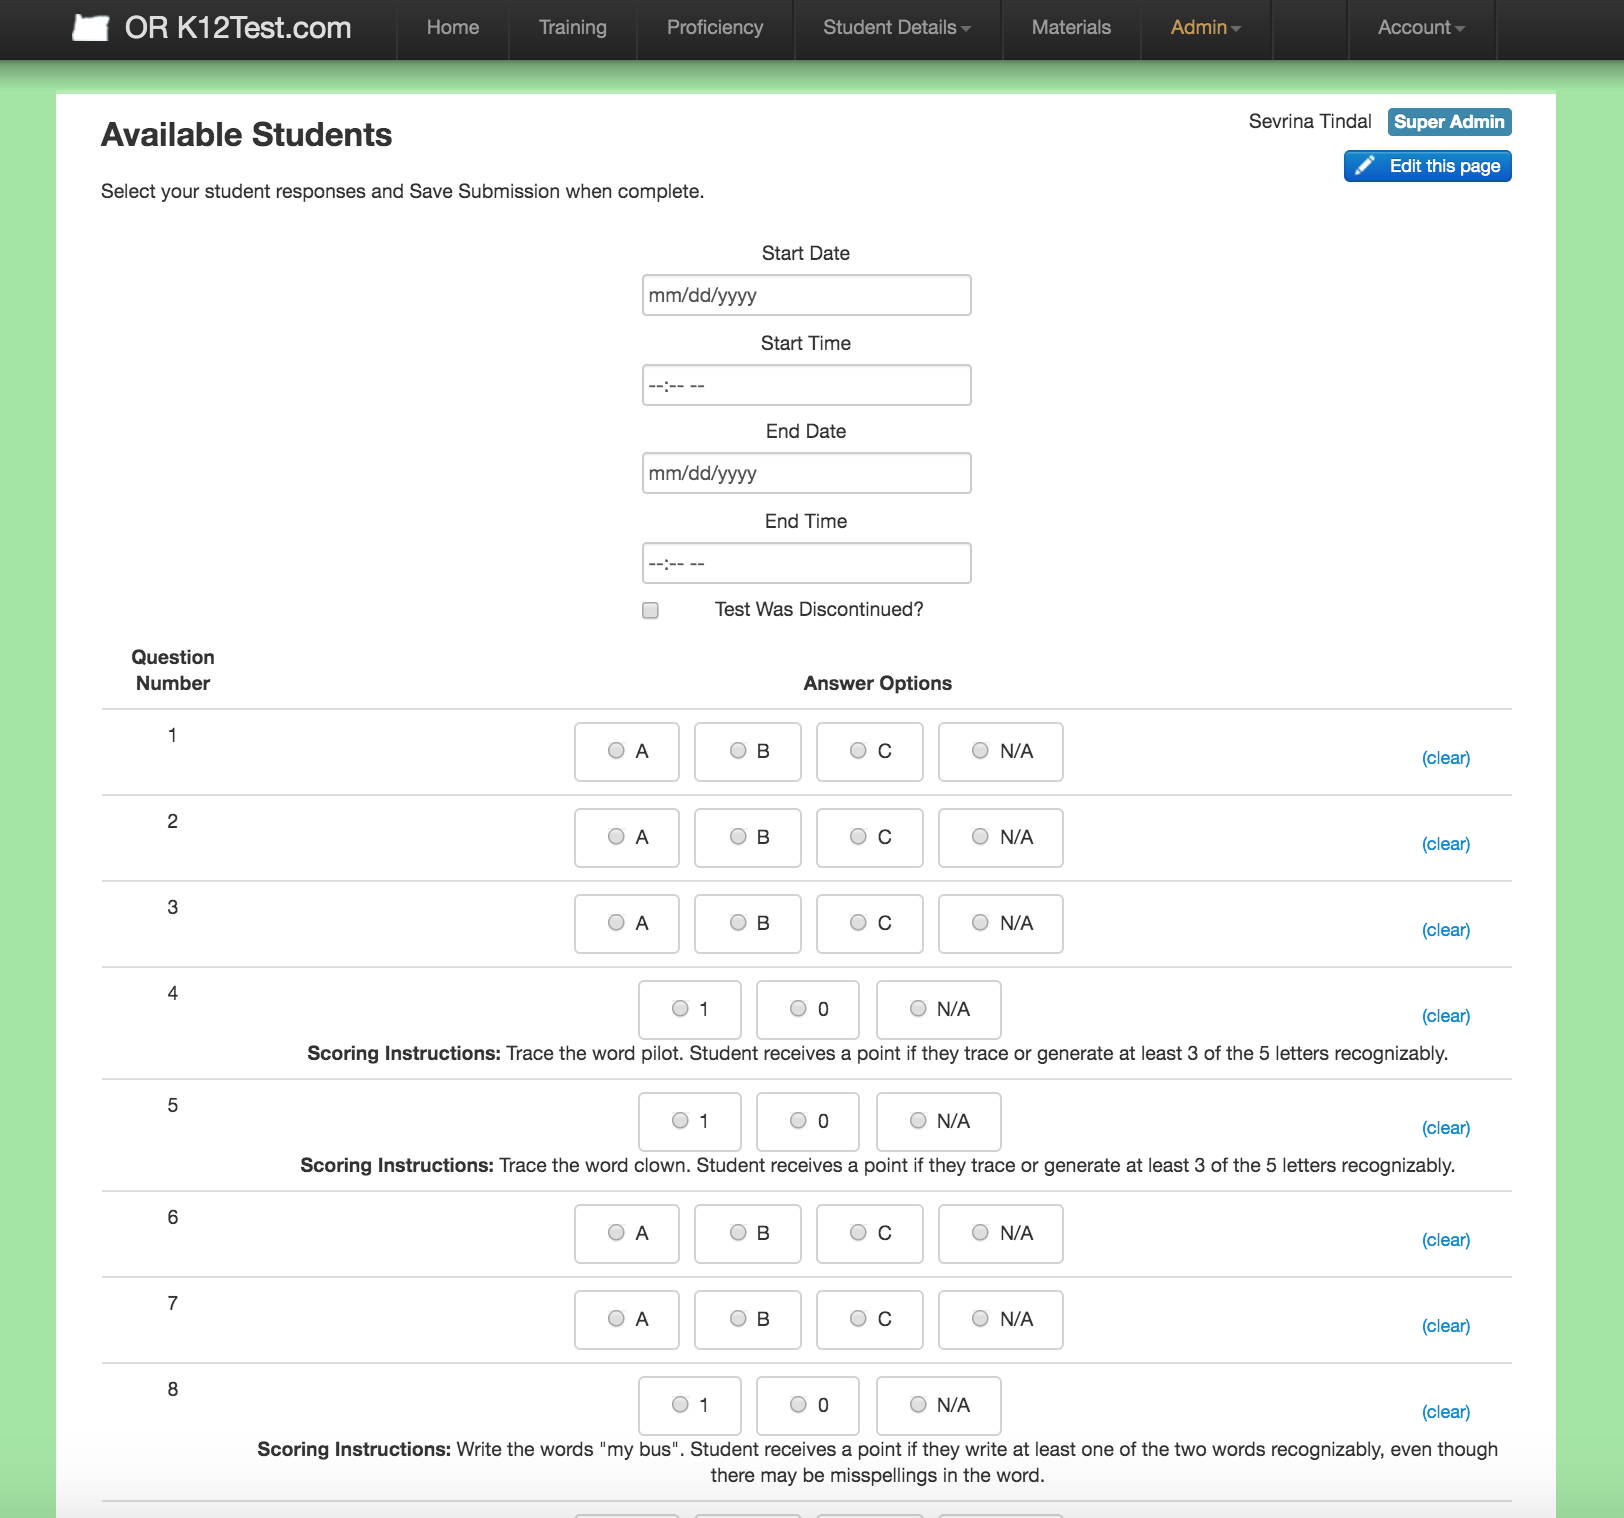
\includegraphics{Figures/TrainingSite/DataEntryPg.png}

\hypertarget{b-secure-student-level-assessment-data}{%
\paragraph{2.6B Secure Student-Level Assessment
Data}\label{b-secure-student-level-assessment-data}}

Student level datais protected by relevant training and through a secure
data system in which all data entry is conducted online using
password-protected, secure procedures on the \color{link}
\href{https://or.k12test.com}{Oregon K12 website} \color{black} Only
trained users with a vested educational interest who have signed test
security agreements are authorized to access to online data entry
systems.

\hypertarget{c-protecting-personally-identifiable-information}{%
\paragraph{2.6C Protecting Personally Identifiable
Information}\label{c-protecting-personally-identifiable-information}}

All confidential, personally identifiable student information is
protected by policy and supported by training (see \emph{Appendix}
1.4.2, p.~26). The minimum number of students necessary to allow
reporting of students and student subgroups varies by rating (i.e.,
achievement, growth, graduation, and school size), by level (i.e.,
school/district/state), and by number of years of assessment data
available. For example, to receive an achievement rating, schools must
have at least 40 tests for the two most recent school years in reading
or mathematics. Alternatively, small schools receive an achievement
rating if they have at least 40 tests over the most recent four years.
If a school does not have at least 40 tests over a four-year period,
they will not receive an achievement score (see \emph{Appendix} 2.6C).
Similar rules are applied to student subgroups, including students with
disabilities, English learners, and students from diverse racial/ethnic
backgrounds (see \emph{Appendix} 2.6C, p.~7).


\end{document}
